\section{弹性布局}

弹性布局是浮动布局的替代方案,Flexbox 全称弹性盒子布局(Flexible Box Layout),跟浮动布局相比,Flexbox的可预测性更好,还能提供更精细的控制。

Flexbox 唯一不算缺陷的缺陷是引入了很多新的属性: 12 种。

\subsection{弹性容器基础}

\subsubsection*{弹性布局原则}

使用弹性布局需要给元素添加 \texttt{display: flex} 标签。该元素变成了一个弹性容器(flex container),它的直接子元素变成了弹性子元素(flex item)。
\begin{itemize}
    \item 弹性子元素: 默认在同一行从左到右的顺序并排排列。高度相等,由内容决定。
    \item 弹性容器: 像块元素一样填满可用宽度。
\end{itemize}

\fbox{
    \parbox{0.87\textwidth}{
        \begin{remark}
            可以使用 \texttt{display: inline-flex}。和 \texttt{flex} 唯一的区别是宽度不会占满视口。\texttt{display} 的其他值 \texttt{block, inline-block} 只影响对应的元素,但弹性布局会控制内部的元素。
        \end{remark}
    }
}

子元素按照主轴线排列,主轴的方向为主起点(左)到主终点(右)。垂直于主轴的是副轴。方向从副起点(上)到副终点(下)。主轴与副轴的方向可以改变。

\begin{figure}[H]
    \small
    \centering
    \begin{tikzpicture}[scale = 1]
        \draw[color = white, fill = black!10] (0,0) rectangle (7.5,2);
        \foreach \i in {1,2,3,4} {
            \node[fill = black!40, font = \large, inner sep = 1em] (\i) at (\i*1.5,1) {\i};
        }
        \draw [-Stealth] (-0.25, 2) -- (-0.25,0) node [midway, left] {副轴};
        \draw [-Stealth] (0, 2.25) -- (7.5,2.25) node [midway, above] {主轴};
    \end{tikzpicture}
    \caption{弹性元素}
    \label{fig:弹性元素}
\end{figure}

\subsubsection*{弹性子元素的大小}

一般我们使用 \texttt{width, height} 属性设置元素的大小,但是 Flexbox 提供了更强大的属性: \texttt{flex}, \texttt{flex} 可以用简写,该属性包含了以下三个属性(依次为: \texttt{flex-grow, flex-shrink, flex-grow}):
\begin{itemize}
    \item \texttt{flex-basis}: 定义了元素大小的基准值,即一个初始的“主尺寸”。\texttt{flex-basis}属性可以设置为任意的\texttt{width}值,包括\texttt{px、em}、百分比。它的初始值是\texttt{auto},此时浏览器会检查元素是否设置了\texttt{width}属性值。如果有,则使用\texttt{width}的值作为\texttt{flex-basis}的值;如果没有,则用元素内容自身的大小。如果\texttt{flex-basis}的值不是\texttt{auto},\texttt{width}属性会被忽略。
\begin{figure}[H]
    \small
    \centering
    \begin{tikzpicture}[scale = 1,ultra thick]
        \draw [color = white, fill = black!10] (-0.25,-0.25) rectangle (10.25,1.25);
        \draw [color = black!10, fill = black!40] (0,0) rectangle (2,1);
        \draw [color = black!10, fill = black!40] (2,0) rectangle (4,1);
        \draw [color = black!10, fill = black!40] (4,0) rectangle (6,1);
        \draw [color = black!10, fill = black!20] (6,0) rectangle (10,1);
        \begin{scope}[font = \tiny]
            \node [] at (1,0.5) {\texttt{flex-basic: 20\%}};
            \node [] at (3,0.5) {\texttt{flex-basic: 20\%}};
            \node [] at (5,0.5) {\texttt{flex-basic: 20\%}};
            \node [] at (8,0.5) {剩余 \texttt{40\%}};
        \end{scope}
    \end{tikzpicture}
    \caption{flex-basis}
    \label{fig:flex-basis}
\end{figure}
每个弹性子元素的初始主尺寸确定后,它们可能需要在主轴方向扩大或者缩小来适应(或者填充)弹性容器的大小。这时候就需要\texttt{flex-grow}和\texttt{flex-shrink}来决定缩放的规则。
    \item \texttt{flex-grow}: 每个弹性子元素的\texttt{flex-basis}值计算出来后,它们(加上子元素之间的外边距)加起来会占据一定的宽度。加起来的宽度不一定正好填满弹性容器的宽度,可能会有留白.多出来的留白(或剩余宽度)会按照\texttt{flex-grow}(增长因子)的值按比例分配给每个弹性子元素。
\begin{figure}[H]
    \small
    \centering
    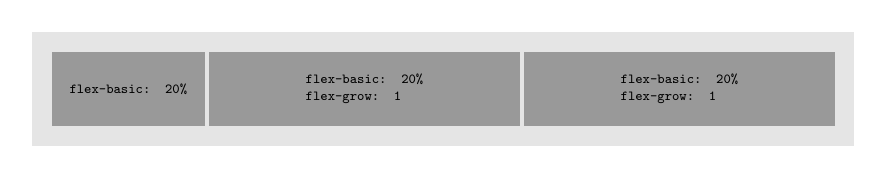
\begin{tikzpicture}[scale = 1,ultra thick]
        \draw [color = white, fill = black!10] (-0.25,-0.25) rectangle (10.25,1.25);
        \draw [color = black!10, fill = black!40] (0,0) rectangle (2,1);
        \draw [color = black!10, fill = black!40] (2,0) rectangle (6,1);
        \draw [color = black!10, fill = black!40] (6,0) rectangle (10,1);
        \begin{scope}[font = \tiny]
            \node [] at (1,0.5) {\texttt{flex-basic: 20\%}};
            \node [align = left] at (4,0.5) {\texttt{flex-basic: 20\%} \\ \texttt{flex-grow: 1}};
            \node [align = left] at (8,0.5) {\texttt{flex-basic: 20\%} \\ \texttt{flex-grow: 1}};
        \end{scope}
    \end{tikzpicture}
    \caption{flex-growth}
    \label{fig:flex-growth}
\end{figure}
    \item \texttt{flex-shrink}: 前两个属性都是对于盒模型宽度来说的,如果 \texttt{margin} 设置的过大,容器内的元素完全有可能超出范围,因此需要 \texttt{flex-shrink} 来收缩,收缩的算法和 \texttt{flex-grow} 相同。
\end{itemize}

\texttt{flex} 属性最后两个值默认是 \texttt{flex-shrink: 1, flex-grow: 0\%}。最好使用 \texttt{flex} 而不是精确的 \texttt{flex-xxx},因为这样会有后两个属性的默认值。

\subsubsection*{弹性方向}

在使用弹性布局时,同一容器内元素的高度是相同的,但有时会出现如下的情况:

\begin{figure}[H]
    \small
    \centering
    
\begin{tikzpicture}[scale = 1,ultra thick]
        \draw[color=white, fill=black!40] (0,0) rectangle (2,2);
        \draw[color=white, fill=black!40] (2,1) rectangle (3,2);
        \draw[color=white, fill=black!40] (2,0.5) rectangle (3,1);
    \end{tikzpicture}
    \caption{弹性布局板块高度不一致}
    \label{fig:弹性布局板块高度不一致}
\end{figure}

左右两列为弹性布局容器中的两个元素,虽然两个子元素是等高的,但是右边栏内部的两个板块没有扩展到填满右边栏区域。

对应的解决方案是将右侧子元素设置为弹性容器,并改变弹性方向(\texttt{flex-direction}):

\begin{HTML}
.column2 {
    display: flex;
    flex-direction: column;
}
\end{HTML}

同时将右侧的两个元素加上 \texttt{flex-growth}:

\begin{HTML}
.element1 .element2 {
    flex: 1;
}
\end{HTML}

这样,两个子元素就会自动在竖直方向上填充。

\subsection{弹性容器的属性}
\subsubsection*{容器换行}

如果界面缩的很小,由于弹性元素的部分内容会占固定的宽度(即最小宽度), 这时候部分内容可能就会超出屏幕范围,如果不想这样,可以使用 \texttt{flex-wrap} 属性。

\begin{figure}[H]
    \small
    \centering
    \begin{minipage}[t]{0.4\linewidth}
        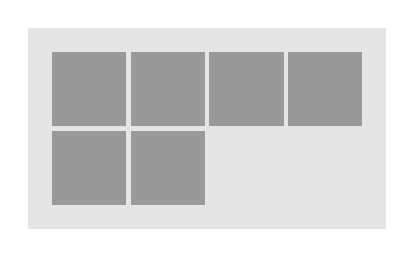
\begin{tikzpicture}[scale = 1,ultra thick]
            \draw[color = black!10, fill=black!10] (-0.25,-0.25) rectangle (4.25,2.25);
            \draw[color = black!10, fill=black!40] (0,1) rectangle (1,2);
            \draw[color = black!10, fill=black!40] (1,1) rectangle (2,2);
            \draw[color = black!10, fill=black!40] (2,1) rectangle (3,2);
            \draw[color = black!10, fill=black!40] (3,1) rectangle (4,2);
            \draw[color = black!10, fill=black!40] (0,0) rectangle (1,1);
            \draw[color = black!10, fill=black!40] (1,0) rectangle (2,1);
        \end{tikzpicture}
        \texttt{wrap}
    \end{minipage}\qquad
    \begin{minipage}[t]{0.4\linewidth}
        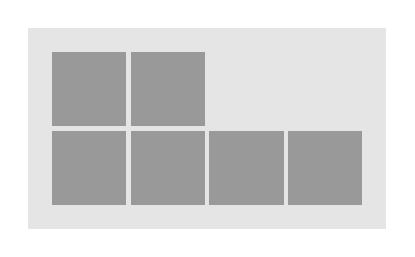
\begin{tikzpicture}[scale = 1,ultra thick]
            \draw[color = black!10, fill=black!10] (-0.25,-0.25) rectangle (4.25,2.25);
            \draw[color = black!10, fill=black!40] (0,0) rectangle (1,1);
            \draw[color = black!10, fill=black!40] (1,0) rectangle (2,1);
            \draw[color = black!10, fill=black!40] (2,0) rectangle (3,1);
            \draw[color = black!10, fill=black!40] (3,0) rectangle (4,1);
            \draw[color = black!10, fill=black!40] (0,1) rectangle (1,2);
            \draw[color = black!10, fill=black!40] (1,1) rectangle (2,2);
        \end{tikzpicture}
        \texttt{wrap-reverse}
    \end{minipage}
    \caption{flex-direction}
\end{figure}

默认情况下,\texttt{flex-wrap} 值为 \texttt{nowrap}。如果修改了弹性方向,对应的换行也会改变。

此外,有一个 \texttt{flex-flow} 简写,包含两个值,分别为 \texttt{flex-direction flex-wrap}。

\subsubsection*{容器主轴对齐}

\texttt{justify-content} 用于控制子元素主轴上的位置,主要是针对空白区域的填充方案,默认值为 \texttt{center}。

\begin{figure}[H]
    \small
    \centering
    \begin{minipage}[t]{0.4\linewidth}
        
\begin{tikzpicture}[scale = 1,ultra thick]
            \draw[color = black!10, fill=black!10] (-0.25,-0.25) rectangle (5.25,1.25);
            \draw[color = black!10, fill=black!40] (0,0) rectangle (1,1);
            \draw[color = black!10, fill=black!40] (1,0) rectangle (2,1);
            \draw[color = black!10, fill=black!40] (2,0) rectangle (3,1);
        \end{tikzpicture}
        \texttt{flex-start}
    \end{minipage}
    \begin{minipage}[t]{0.4\linewidth}
        
\begin{tikzpicture}[scale = 1,ultra thick]
            \draw[color = black!10, fill=black!10] (-0.25,-0.25) rectangle (5.25,1.25);
            \draw[color = black!10, fill=black!40] (2,0) rectangle (3,1);
            \draw[color = black!10, fill=black!40] (3,0) rectangle (4,1);
            \draw[color = black!10, fill=black!40] (4,0) rectangle (5,1);
        \end{tikzpicture}
        \texttt{flex-end}
    \end{minipage}
    \begin{minipage}[t]{0.4\linewidth}
        
\begin{tikzpicture}[scale = 1,ultra thick]
            \draw[color = black!10, fill=black!10] (-0.25,-0.25) rectangle (5.25,1.25);
            \draw[color = black!10, fill=black!40] (0,0) rectangle (1,1);
            \draw[color = black!10, fill=black!40] (2,0) rectangle (3,1);
            \draw[color = black!10, fill=black!40] (4,0) rectangle (5,1);
        \end{tikzpicture}
        \texttt{space-between}
    \end{minipage}
    \begin{minipage}[t]{0.4\linewidth}
        
\begin{tikzpicture}[scale = 1,ultra thick]
            \draw[color = black!10, fill=black!10] (-0.25,-0.25) rectangle (5.25,1.25);
            \draw[color = black!10, fill=black!40] (0.5,0) rectangle (1.5,1);
            \draw[color = black!10, fill=black!40] (2,0) rectangle (3,1);
            \draw[color = black!10, fill=black!40] (3.5,0) rectangle (4.5,1);
        \end{tikzpicture}
        \texttt{space-around}
    \end{minipage}
    \begin{minipage}[t]{0.4\linewidth}
        
\begin{tikzpicture}[scale = 1,ultra thick]
            \draw[color = black!10, fill=black!10] (-0.25,-0.25) rectangle (5.25,1.25);
            \draw[color = black!10, fill=black!40] (1,0) rectangle (2,1);
            \draw[color = black!10, fill=black!40] (2,0) rectangle (3,1);
            \draw[color = black!10, fill=black!40] (3,0) rectangle (4,1);
        \end{tikzpicture}
        \texttt{center}
    \end{minipage}
    \caption{flex-direction}
\end{figure}

\subsubsection*{容器副轴对齐}

\texttt{align-items} 用于控制副轴上的位置,默认值为 \texttt{stretch}。值和 \texttt{justify-content} 类似,\texttt{stretch} 会拉伸元素高度,\texttt{baseline} 则以字体的下划线位置对齐。

\subsubsection*{开启换行后多行元素对齐}

\texttt{align-content} 需要开启 \texttt{flex-wrap} 能使用,将每一行多个元素当作单个元素看,效果就是副轴上的 \texttt{justify-content} 和 \texttt{text-align} 结合。

\subsubsection*{弹性元素的属性}

除了前面提到的 \texttt{flex},弹性元素属性只有两个: 

\begin{itemize}
    \item \texttt{align-self}: 用于控制单个元素的 \texttt{align-item} 对齐方案,值和 \texttt{align-item} 一致。
    \item \texttt{Order}: 用于改变 HTML 中元素的顺序,不是很推荐使用。
\end{itemize}

\newpage